\documentclass{report}
\usepackage{multicol,multirow}
\usepackage{amsfonts,amssymb,amsmath,wasysym,amsthm}
\usepackage{fancybox}
\usepackage{graphicx}
\usepackage[left=2cm,right=1.5cm,bottom=1.5cm,top=2.25cm]{geometry}
\usepackage[utf8]{inputenc}
\usepackage{hyperref}
\usepackage{listings}
\begin{document}
	\thispagestyle{empty}
\begin{tabular}{l c r}

\includegraphics[scale=0.5]{ucv.jpg} &
\begin{minipage}{10cm}
\centering
\vspace{-2.5cm}
\bf{ \large {Universidad Central De Venezuela\\
			Facultad De Ciencias \\
			Escuela De Computación \\\
			Introducción a la Ciencia de Datos}} \\
	\vspace{4mm}
	\shadowbox{\bf {Proyecto}}
\end{minipage} &

\includegraphics[height=2.7cm,width=2.5cm,scale=0.1]{ciencias.jpg}
\end{tabular}
\vspace{7cm}
\begin{center}
	\Huge{\textbf{Técnica de regresión para la predicción de precios de viviendas}} \linebreak
	\linebreak
	\Large{Br. José Castillo} \Large{C.I: V-24.636.302} \linebreak
	\Large{Br. Yoselin Arvelaiz} \Large{C.I: V-22.887.653} 
\end{center}
\newpage
\setcounter{page}{1}

\begin{itemize}
\item \textbf{\large{\underline{Introducción y motivación}}}
\vspace{2mm}

Aprender y conocer como se desarrolla la Ciencia de Datos es nuestra principal motivación. En la vida díaria muchas veces nos hemos preguntado el costo de una vivienda en diversas condiciones ya sea que tenga garage, sótano, cobertizo, entre otros y es por esto que tomamos la iniciativa de comenzar a realizar Ciencia de Datos.\\ \\
El objetivo principal de este proyecto es aplicar técnicas de regresión para predecir el precio de venta de la propiedad residencial en Ames, Iowa.Iniciaremos con la limpieza de los datos analizando los valores faltantes.luego, haremos un análisis exploratorio en algunas variables y finalmente aplicaremos el módelo de regresión.\\

\item \textbf{\large{\underline{Antecedentes}}}
\vspace{2mm}

Nos hemos inspirado y guiado en trabajos realizados en la página web: \url{www.kaggle.com}.\\

\item \textbf{\large{\underline{Datos}}}
\vspace{2mm}

\begin{itemize}
\item[1.] \textbf{\underline{Fuente de Datos:}}\\

Los datos fueron extraídos de \url{www.kaggle.com/c/house-prices-advanced-regression-techniques}.\\

\item[2.] \textbf{\underline{Limpieza de Datos:}}\\ \\
Lo primero que hicimos fue descargar los datos de entrenamiento y prueba, donde los datos de entrenamiento tienen 1460 observaciones con 81 variables y los datos de prueba tienen 1459 observaciones con 80 variables (excluyendo la variable SalePrice que es la que intentaremos predecir).Combinaremos esta dos datas para un análisis completo y luego separar estas para entrenar el modelo.\\

\lstset{language=R, breaklines=true, basicstyle=\footnotesize}
\begin{lstlisting}[frame=single]
library('ggplot2')
library('scales')
library('corrplot')
train<-read.csv('train.csv',sep=',',header=TRUE)
test<-read.csv('test.csv',sep=',',header=TRUE)
#Anadimos la columna SalePrice a la data de prueba
SalePrice<-rep(NA,times=nrow(test))
d<-cbind(SalePrice,test)
f<-rbind(train,d)   
dim(f)
\end{lstlisting}  

\begin{lstlisting}[frame=single]
[1] 2919   81
\end{lstlisting} 
\vspace{2mm}

Nuestro conjunto de datos está lleno de muchos valores perdidos, por lo tanto, antes de poder construir cualquier modelo predictivo, limpiaremos nuestros datos rellenando algunos NA con los valores apropiados.Veamos la cantidad de NA's por cada variables: \\

\begin{lstlisting}[frame=single]
s<-data.frame(sapply(f,is.na))
c<-colSums(s,na.rm=TRUE)
Data.faltante<-sort(c[c>0],decreasing = TRUE)
\end{lstlisting}

\newpage
\begin{lstlisting}[frame=single]
 PoolQC  MiscFeature        Alley        Fence    SalePrice  FireplaceQu 
 2909         2814         2721         2348         1459         1420 
 LotFrontage  GarageYrBlt GarageFinish   GarageQual   GarageCond   GarageType 
 486          159          159          159          159          157 
 BsmtCond BsmtExposure     BsmtQual BsmtFinType2 BsmtFinType1   MasVnrType 
 82           82           81           80           79           24 
 MasVnrArea     MSZoning    Utilities BsmtFullBath BsmtHalfBath   Functional 
 23            4            2            2            2            2 
 Exterior1st  Exterior2nd   BsmtFinSF1   BsmtFinSF2    BsmtUnfSF  TotalBsmtSF 
 1            1            1            1            1            1 
 Electrical  KitchenQual   GarageCars   GarageArea     SaleType 
 1            1            1            1            1 
\end{lstlisting}
\vspace{2mm}

Ahora analicemos estas variables en este orden.\\

\begin{itemize}
\item[2.1] \textbf{\underline{PoolQC:}}\\ \\
\begin{figure}[h]
	\centering
	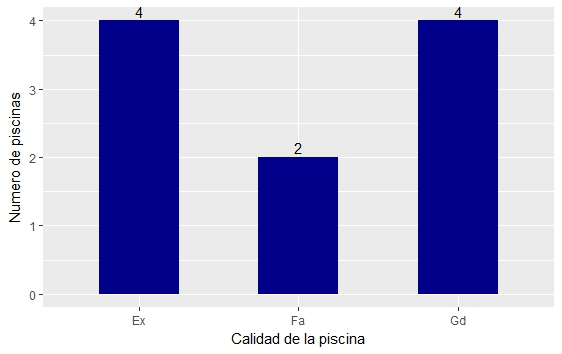
\includegraphics[scale=0.8]{Piscina.JPEG}
	\label{p1}
	\caption{PoolQC}
\end{figure} \\

\begin{lstlisting}[frame=single]
#Veamos cuales de las viviendas tienen piscinas pero no tienen una calidad asociada

f[which(f$PoolArea>0 & is.na(f$PoolQC)),c('PoolArea','PoolQC')]
\end{lstlisting}

\begin{lstlisting}[frame=single]
      PoolArea PoolQC
2421      368   <NA>
2504      444   <NA>
2600      561   <NA>
\end{lstlisting}
\vspace{2mm}

Rellenemos estos valores sacandole la media al area de piscinas asociadas a las piscinas de calidades excelentes,buenas y regulares.\\

\begin{lstlisting}[frame=single]
[1] 359.75 'Ex'    648.5 'Gd'    583.5 'Fa'
\end{lstlisting}

\begin{lstlisting}[frame=single]
f[2421,'PoolQC']='Ex'
f[2504,'PoolQC']='Ex'
f[2600,'PoolQC']='Fa'
\end{lstlisting}

\newpage

\item[2.2] \textbf{\underline{MiscFeature:}}\\ 

Relacionemos MiscFeature con MiscVal.\\

\begin{lstlisting}[frame=single]
#Veamos si las variedades de las viviendas tienen sus precios respectivos y si tienen precios sin variedad

[1] table(f$MiscFeature)

[2] which(f$MiscVal>0 & is.na(f$MiscFeature))

[3] f[2550,c('MiscFeature','MiscVal')]

[4] f[which(f$MiscVal==0 & !is.na(f$MiscFeature)),c('MiscFeature','MiscVal')]
\end{lstlisting}

\begin{lstlisting}[frame=single]
[1]   Gar2 Othr Shed TenC 
       5    4   95    1 

[2] 2550

[3]      MiscFeature MiscVal
2550        <NA>   17000

[4]   MiscFeature MiscVal
874         Othr       0
1201        Shed       0
2432        Shed       0
\end{lstlisting}
\vspace{2mm}

Rellenamos estos valores con la media del precio de las variedades respectivas.\\

\begin{lstlisting}[frame=single]
[1] 4333.333 'Othr' 780.2258 'Shed'  8760 'Gar2' 2000 'TenC'
\end{lstlisting}

\begin{lstlisting}[frame=single]
f[874,'MiscVal']=433
f[1201,'MiscVal']=780
f[2432,'MiscVal']=780
f[2550,'MiscFeature']='Gar2'
\end{lstlisting}

\begin{figure}[h]
	\centering
	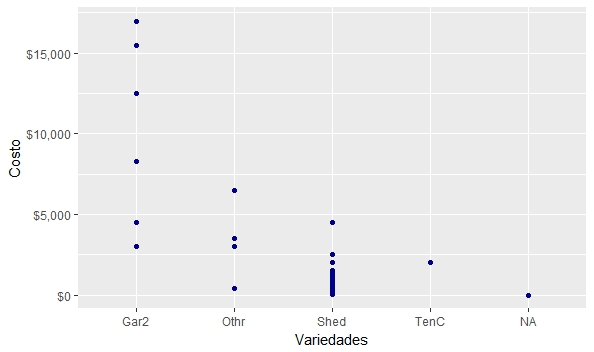
\includegraphics[scale=0.8]{Variedades.JPEG}
	\label{p1}
	\caption{MiscFeature}
\end{figure}

\newpage

\item[2.3] \textbf{\underline{Alley}} \\ 

Se tienen 2721 viviendas sin acceso a un callejón,es decir, hay 198 viviendas con acceso a un callejón pavimentado o de granza. \\

\begin{figure}[h]
	\centering
	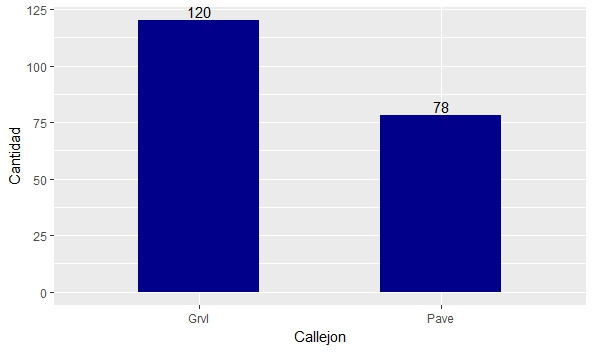
\includegraphics[scale=0.8]{Callejon.JPEG}
	\label{p1}
	\caption{Alley}
\end{figure}


\item[2.4] \textbf{\underline{Fence}}\\

Se tienen 571 viviendas con cercas y 2348 que no tienen. \\

\begin{figure}[h]
	\centering
	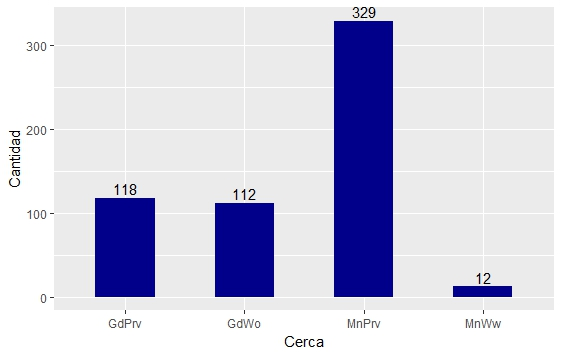
\includegraphics[scale=0.8]{Cerca.JPEG}
	\label{p1}
	\caption{Fence}
\end{figure}

Observamos que hay 118 cercas con buena privacidad,112 con buena madera,329 con poca privacidad y 12 con madera de mala calidad.

\newpage

\item[2.5] \textbf{\underline{FireplaceQU}}\\

Relacionemos la calidad de las chimeneas con la cantidad de chimeneas.\\

\begin{lstlisting}[frame=single]
[1] which(f$Fireplaces>0 & is.na(f$FireplaceQu))
[2] which(f$Fireplaces==0 & !is.na(f$FireplaceQu))
\end{lstlisting}

\begin{lstlisting}[frame=single]
[1] integer(0)
[2] integer(0)
\end{lstlisting}

Por lo que 1420 viviendas efectivamente no tienen chimeneas y por lo tanto no tienen una calidad asociada.\\

\begin{figure}[h]
	\centering
	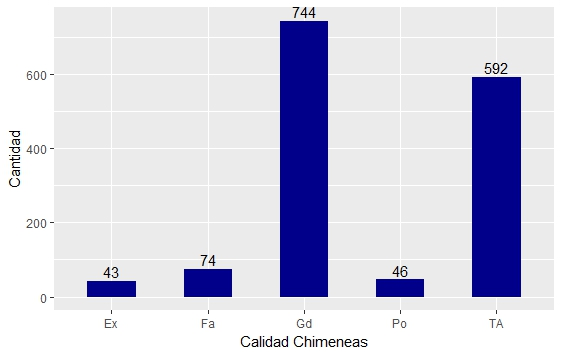
\includegraphics[scale=0.8]{CChimeneas.JPEG}
	\label{p1}
	\caption{FireplaceQU}
\end{figure}

\item[2.6] \textbf{\underline{LotFrontage}}\\

Tenemos 486 valores faltantes para la distancia de la vivienda hasta la calle, lo cual es contradictorio ya que tiene que haber una cierta distancia.Para resolver este problema vamos a relacionar esta distancia con los vecindarios respectivos de cada vivienda.

\begin{lstlisting}[frame=single]
h<-f[order(f$Neighborhood),c('Neighborhood','LotFrontage')]
h1<-h[!is.na(h$LotFrontage),]
h2<-aggregate(h1[,2],list(h1$Neighborhood),median)
h2
\end{lstlisting}

\begin{lstlisting}[frame=single]
     Group.1    x
   1  Blmngtn 43.0
   2  Blueste 24.0
   3   BrDale 21.0
   4  BrkSide 51.0
   5  ClearCr 80.5
   6  CollgCr 70.0
   7  Crawfor 70.0
   8  Edwards 65.0
   9  Gilbert 64.0
   10  IDOTRR 60.0
   11 MeadowV 21.0
   12 Mitchel 74.0
   13   NAmes 73.0
   14 NoRidge 89.0
   15 NPkVill 24.0
\end{lstlisting}   
\begin{lstlisting}[frame=single]
   16 NridgHt 92.0
   17  NWAmes 80.0
   18 OldTown 60.0
   19  Sawyer 72.0
   20 SawyerW 67.0
   21 Somerst 72.5
   22 StoneBr 60.0
   23   SWISU 60.0
   24  Timber 82.0
   25 Veenker 80.0
\end{lstlisting}
\vspace{2mm}

Para rellenar los siguientes valores faltantes los rellenamos con las medianas de sus vecindarios respectivos. 

\begin{lstlisting}[frame=single]
for(i in 1:nrow(f)){if(is.na(f[i,'LotFrontage']))f[i,'LotFrontage']<-h2$x[f[i,'Neighborhood']]}
\end{lstlisting}
\vspace{2mm}

Veamos el antes y despues de haber añadido los nuevos valores para verificar si se sigue manteniendo la distribucion de los datos.\\

\begin{figure}[h]
	\centering
	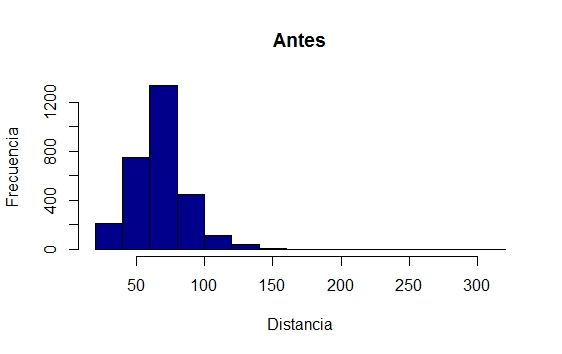
\includegraphics[scale=0.75]{Distancia1.JPEG}
	\label{p1}
	\caption{LotFrontage}
\end{figure}

\begin{figure}[h]
\centering
	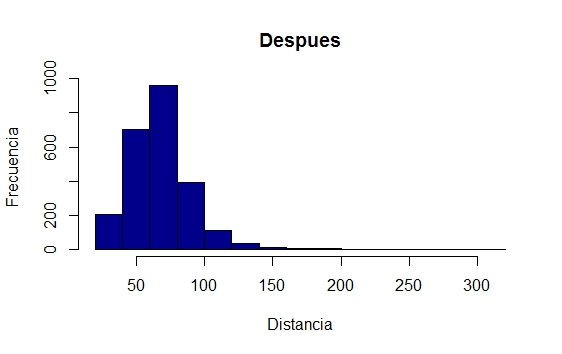
\includegraphics[scale=0.7]{Distancia2.JPEG}
	\label{p1}
	\caption{LotFrontage}
\end{figure}

\newpage

\item[2.7] \textbf{\underline{Garages}}\\

Primero trabajaremos con el año de construcción del garage,ya que se tiene 159 valores faltantes,para esto vamos a relacionarlo con el año de construcción de la vivienda.\\

\begin{lstlisting}[frame=single]
length(which(f$YearBuilt==f$GarageYrBlt))
\end{lstlisting}

\begin{lstlisting}[frame=single]
[1] 2216
\end{lstlisting}
\vspace{2mm}

Por lo que hay 2216 viviendas que coinciden con su año de construcción y el año de construcción del garage.Por ende rellaneremos los 159 valores faltantes con el mismo año de construcción de la respectiva vivienda.\\

Ahora trabajaremos con la variable GarageArea y la relacionaremos con el resto de las variables asociadas a garages.\\

\begin{lstlisting}[frame=single]
[1] which(f$GarageArea>0 & (f$GarageCars==0 | is.na(f$GarageCars)))
[2] which(f$GarageArea>0 & is.na(f$GarageType))

[3] which(f$GarageArea>0 & is.na(f$GarageQual))
[4] which(f$GarageArea>0 & is.na(f$GarageFinish))
[5] which(f$GarageArea>0 & is.na(f$GarageCond))
\end{lstlisting}

\begin{lstlisting}[frame=single]
[1] integer(0)
[2] integer(0)

[3] 2127
[4] 2127
[5] 2127
\end{lstlisting}
\vspace{2mm}

Podemos observar que en la fila 2127 existe un área de garage pero no tiene una calidad, condición o si esta terminado o no, por otra parte la variable GarageArea tiene un solo valor faltante, veamos si esta tiene una inconsistencia. Llamemos estas dos filas.\\

\begin{lstlisting}[frame=single]
f[c(2127,which(is.na(f$GarageArea))),c('GarageArea','GarageCars','GarageQual','GarageFinish','GarageCond','GarageType')]
\end{lstlisting}

\begin{lstlisting}[frame=single]
      GarageArea  GarageCars    GarageQual  GarageFinish  GarageCond  GarageType
2127    360          1           <NA>          <NA>          <NA>       Detchd
2577     NA         NA           <NA>          <NA>          <NA>       Detchd
\end{lstlisting}
\vspace{2mm}

Para resolver esto hicimos lo siguiente.\\

\begin{lstlisting}[frame=single]
na2<-which(f$GarageArea==360 & f$GarageCars==1)
f[na2,c('GarageArea','GarageCars','GarageQual','GarageFinish','GarageCond','GarageType')]
\end{lstlisting}

\begin{lstlisting}[frame=single]
        GarageArea GarageCars GarageQual GarageFinish GarageCond GarageType
 463         360          1         TA          Unf         TA     Detchd
 2127        360          1       <NA>         <NA>       <NA>     Detchd
 2215        360          1         TA          RFn         TA     Detchd
 2286        360          1         TA          Unf         TA     Detchd
 2588        360          1         TA          Unf         TA     Attchd
 2861        360          1         TA          Unf         TA     Attchd
\end{lstlisting}
\vspace{2mm}

Asi para la fila 2127 rellenamos los valores faltantes con las categorias que mas se repiten que son 'TA', 'Unf' y 'TA'. Para la fila 2577 que tiene un valor incosistente lo rellenamos con NA y a los valores GarageArea y GarageCars con cero.\\
\begin{lstlisting}[frame=single]
f[2127,'GarageQual']<-'TA'
f[2127,'GarageFinish']<-'Unf'
f[2127,'GarageCond']<-'TA'

f[2577,'GarageType']<-NA
f[2577,c('GarageArea','GarageCars')]<-0
\end{lstlisting}
\vspace{2mm}

\item[2.8] \textbf{\underline{Bsmt}}\\

Primero trabajaremos con la condición del sótano donde se tienen 82 valores faltantes.\\

\begin{lstlisting}[frame=single]
Bsmt<-c('BsmtQual','BsmtCond','BsmtExposure','BsmtFinType1','BsmtFinSF1','BsmtFinType2','BsmtFinSF2','BsmtUnfSF','TotalBsmtSF','BsmtFullBath','BsmtHalfBath')

A<-f[which(is.na(f$BsmtCond)),Bsmt]
A[which(A$TotalBsmtSF>0),]
\end{lstlisting}
\vspace{2mm}
Veamos si existe un área de sótano y no tenga una condición asociada.\\
\begin{lstlisting}[frame=single]
        BsmtQual BsmtCond BsmtExposure BsmtFinType1 BsmtFinSF1 BsmtFinType2 BsmtFinSF2
2041       Gd     <NA>           Mn          GLQ       1044          Rec        382
2186       TA     <NA>           No          BLQ       1033          Unf          0
2525       TA     <NA>           Av          ALQ        755          Unf          0
        BsmtUnfSF TotalBsmtSF BsmtFullBath BsmtHalfBath
2041         0        1426            1            0
2186        94        1127            0            1
2525       240         995            0            0
\end{lstlisting}
\vspace{2mm}

Tenemos 3 filas con un área de sótano sin una condición, para esto rellenamos estos valores con la que tenga mayor frecuencia.\\

\begin{figure}[h]
	\centering
	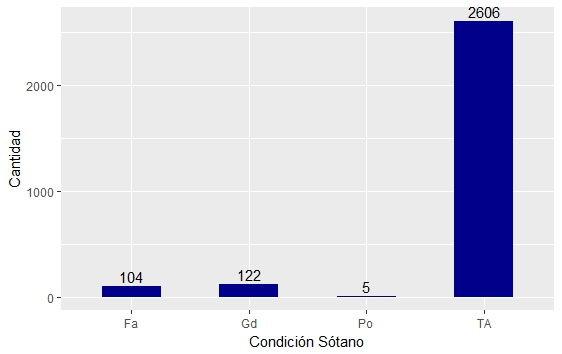
\includegraphics[scale=0.8]{Csotano.JPEG}
	\label{p1}
	\caption{BsmtCond}
\end{figure}

Así,

\begin{lstlisting}[frame=single]
f[2041,'BsmtCond']<-'TA'
f[2186,'BsmtCond']<-'TA'
f[2525,'BsmtCond']<-'TA'
\end{lstlisting}

\newpage

El área de los sótanos tiene un solo valor faltante, veamos.\\

\begin{lstlisting}[frame=single]
f[which(is.na(f$TotalBsmtSF)),Bsmt]
\end{lstlisting}

\begin{lstlisting}[frame=single]
       BsmtQual BsmtCond BsmtExposure BsmtFinType1 BsmtFinSF1 BsmtFinType2 BsmtFinSF2
2121     <NA>     <NA>         <NA>         <NA>         NA         <NA>         NA
          BsmtUnfSF TotalBsmtSF BsmtFullBath BsmtHalfBath
2121        NA          NA           NA           NA
\end{lstlisting}
\vspace{2mm}
BsmtFullBath y BsmtHalfBath tienen dos valores faltantes c/u, y como pudimos observar en la fila 2121 ambos tienen un NA en común, veamos en que fila ellos tienen el NA faltante y si estos coinciden.\\

\begin{lstlisting}[frame=single]
f[which(is.na(f$BsmtFullBath) & is.na(f$BsmtHalfBath)),Bsmt]
\end{lstlisting}

\begin{lstlisting}[frame=single]
       BsmtQual BsmtCond BsmtExposure BsmtFinType1 BsmtFinSF1 BsmtFinType2 BsmtFinSF2
2121     <NA>     <NA>         <NA>         <NA>         NA         <NA>         NA
2189     <NA>     <NA>         <NA>         <NA>          0         <NA>          0
        BsmtUnfSF TotalBsmtSF BsmtFullBath BsmtHalfBath
2121        NA          NA           NA           NA
2189         0           0           NA           NA
\end{lstlisting}
\vspace{2mm}
Notamos que en la fila 2189 ambos tienen el NA que faltaba, asi vamos a rellenar en las filas 2121 y 2189 de ceros a las variables númericas que tienen NA.\\

\begin{lstlisting}[frame=single]
f[2121,c('BsmtFinSF1','BsmtFinSF2','BsmtUnfSF','TotalBsmtSF','BsmtFullBath','BsmtHalfBath')]<-0
f[2189,c('BsmtFullBath','BsmtHalfBath')]<-0
\end{lstlisting}
\vspace{2mm}

BsmtExposure y BsmtCond tienen la misma cantidad de valores faltantes -82-, pudimos observar en la matriz A que BsmtExposure con relación a los NA de BsmtCond no coincidian en 3 filas, es decir, hay 3 valores faltantes en la variable BsmtExposure que tienen una condición,veamos.\\

\begin{lstlisting}[frame=single]
A1<-f[which(is.na(f$BsmtExposure) & !is.na(f$BsmtCond)),Bsmt]
\end{lstlisting}

\begin{lstlisting}[frame=single]
         BsmtQual BsmtCond BsmtExposure BsmtFinType1 BsmtFinSF1 BsmtFinType2 BsmtFinSF2
949        Gd       TA         <NA>          Unf          0          Unf          0
1488       Gd       TA         <NA>          Unf          0          Unf          0
2349       Gd       TA         <NA>          Unf          0          Unf          0
         BsmtUnfSF TotalBsmtSF BsmtFullBath BsmtHalfBath
949        936         936            0            0
1488      1595        1595            0            0
2349       725         725            0            0
\end{lstlisting}
\vspace{2mm}

Rellenemos estos valores faltantes, con las categorías que mas se repiten, veamos.\\

\newpage
\begin{figure}[h]
	\centering
	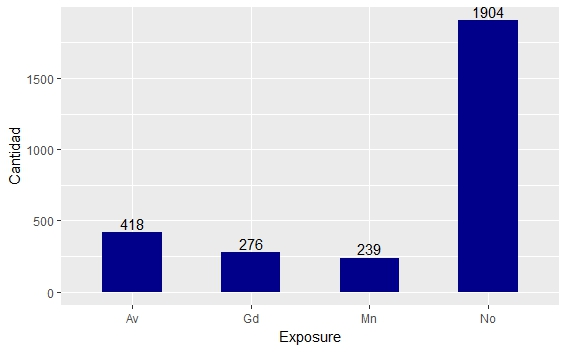
\includegraphics[scale=0.8]{Exposure.JPEG}
	\label{p1}
	\caption{BsmtExposure}
\end{figure}

\begin{lstlisting}[frame=single]
f[c(949,1488,2349),'BsmtExposure']<-'No'
\end{lstlisting}
\vspace{2mm}

Veamos ahora los valores faltantes en la calidad del sótano (BsmtQual).\\

\begin{lstlisting}[frame=single]
A2<-f[which(is.na(f$BsmtQual)),Bsmt]
\end{lstlisting}
\vspace{2mm}

Acá podemos observar que en las filas 2218 y 2219 hay sótanos con condiciones,tipos,etc.. ,para esto busquemos los valores que mas se repiten en esta variable y rellenemosle con estos.\\

\begin{figure}[h]
	\centering
	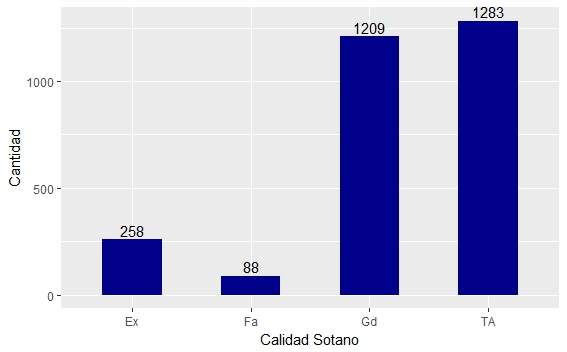
\includegraphics[scale=0.8]{Calidadsotano.JPEG}
	\label{p1}
	\caption{BsmtQual}
\end{figure}

\begin{lstlisting}[frame=single]
f[c(2218,2219),'BsmtQual']<-'TA'
\end{lstlisting}

\newpage

Análogamente hacemos lo mismo con BsmtFinType1 y BsmtFinType2.\\

\begin{lstlisting}[frame=single]
A3<-f[which(is.na(f$BsmtFinType1)),Bsmt]
A4<-f[which(is.na(f$BsmtFinType2)),Bsmt]
\end{lstlisting}
\vspace{2mm}

Aqui podemos observar que en la matriz A3 la variable BsmtFintype1 no tiene problemas ya que los NA estan relacionados con la ausencia de sótanos.Por otro lado en la matriz A4 podemos observar que existe una inconsistencia con la variable BsmtFinType2 en la fila 333. Para resolverlo rellenemosle con la categoría mas frecuente.\\

\begin{figure}[h]
	\centering
	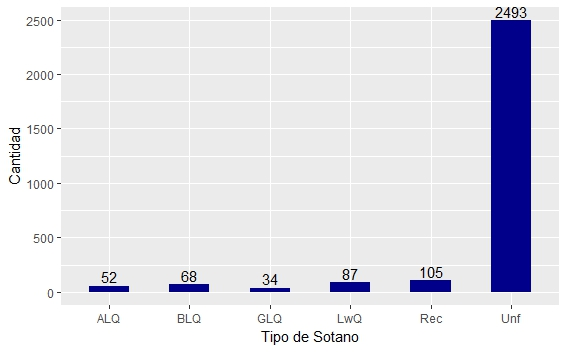
\includegraphics[scale=0.8]{Tiposotano.JPEG}
	\label{p1}
	\caption{BsmtFinType2}
\end{figure}

\begin{lstlisting}[frame=single]
f[333,'BsmtFinType2']<-'Unf'
\end{lstlisting}
\vspace{2mm}

\item[2.9]\textbf{\underline{MasVnrType}}\\

Relacionemos la fachada de las viviendas con el área de las fachadas ya que el tipo de fachada tiene 24 valores faltantes y el área tiene 23.\\

\begin{lstlisting}[frame=single]
V<-f[which(is.na(f$MasVnrType) | is.na(f$MasVnrArea)),c('MasVnrType','MasVnrArea')]
\end{lstlisting}
\vspace{2mm}

Notamos que en la fila 2611 existe un área de fachada de 198 pero que no tiene un tipo, para esto saquemos la mediana de las áreas de los tipos de fachada y le asociamos a la que mejor se ajuste.\\

\begin{lstlisting}[frame=single]
V1<-f[order(f$MasVnrType),c('MasVnrType','MasVnrArea')]
V2<-V1[!is.na(V1$MasVnrType),]
V3<-aggregate(V2[,2],list(V2$MasVnrType),median)
V3
\end{lstlisting}
\vspace{2mm}
Asi las medianas de la área de cada tipo de fachada viene dado por.\\

\begin{lstlisting}[frame=single]
  Group.1   x
1  BrkCmn 161
2 BrkFace 203
3    None   0
4   Stone 200
\end{lstlisting}
\vspace{2mm}

Así como el área de la fachada es de 198 le asociamos la fachada de tipo Stone.\\
\begin{lstlisting}[frame=single]
f[2611,'MasVnrType']<-'Stone'
\end{lstlisting}
\vspace{2mm}

\item[2.10] \textbf{\underline{MSZoning}}\\

Para los 4 valores faltantes de la zona de las viviendas las vamos a relacionar con el tipo de vivienda.\\

\begin{lstlisting}[frame=single]
[1] f[is.na(f$MSZoning),c('MSZoning','MSSubClass')]
[2] table(f$MSZoning,f$MSSubClass)
\end{lstlisting}

\begin{lstlisting}[frame=single]
[1]       MSZoning MSSubClass
1916     <NA>         30
2217     <NA>         20
2251     <NA>         70
2905     <NA>         20

[2]        20   30   40   45   50   60   70   75   80   85   90  120  150  160  180  190
C (all)    3    8    0    0    7    0    4    0    0    0    0    0    0    0    0    3
FV        34    0    0    0    0   43    0    0    0    0    0   19    0   43    0    0
RH         4    2    0    1    2    0    3    0    0    0    4    6    0    0    0    4
RL      1016   61    4    6  159  529   57    9  115   47   92  117    1   21    0   31
RM        20   67    2   11  119    3   63   14    3    1   13   40    0   64   17   23
\end{lstlisting}

\begin{lstlisting}[frame=single]
f[c(2217,2905),'MSZoning']<-'RL'
f[c(1916,2251),'MSZoning']<-'RM'
\end{lstlisting}
\vspace{2mm}

\item[2.11] \textbf{\underline{Utilities}}\\

En los servicios de las viviendas tenemos dos valores faltantes, veamos en que filas de nuestra data se encuentran.\\

\begin{lstlisting}[frame=single]
which(is.na(f$Utilities))
\end{lstlisting}
\begin{lstlisting}[frame=single]
[1] 1916 1946
\end{lstlisting}
\vspace{2mm}

Veamos cuáles son los valores que se repiten más y rellenemosle con estos.\\


\begin{figure}[h]
	\centering
	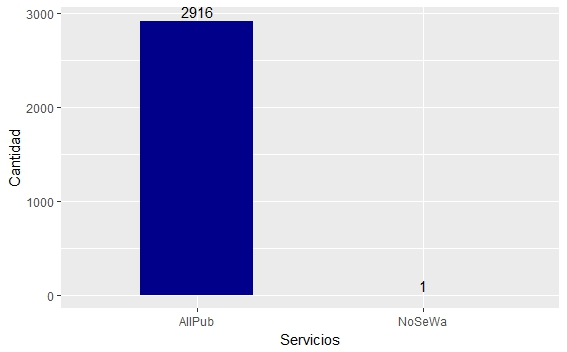
\includegraphics[scale=0.7]{Servicios.JPEG}
	\label{p1}
	\caption{Utilities}
\end{figure}

\newpage

\begin{lstlisting}[frame=single]
f[c(1916,1946),'Utilities']<-'AllPub'
\end{lstlisting}
\vspace{2mm}

\item[2.12] \textbf{\underline{Functional}}\\

Análogamente como hicimos en la variable servicios tenemos: \\

\begin{lstlisting}[frame=single]
which(is.na(f$Functional))
\end{lstlisting}
\begin{lstlisting}[frame=single]
[1] 2217 2474
\end{lstlisting}
\vspace{2mm}

Veamos cuáles son los valores que se repiten más y rellenemosle con estos.\\


\begin{figure}[h]
	\centering
	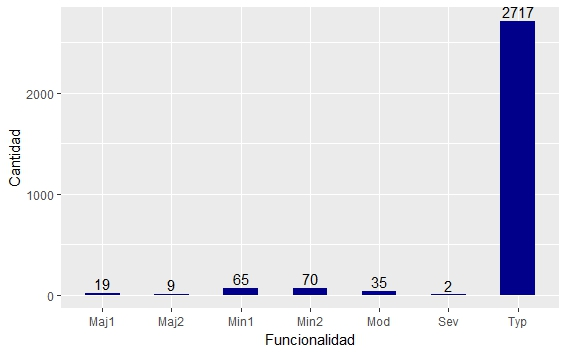
\includegraphics[scale=0.8]{Funcionalidad.JPEG}
	\label{p1}
	\caption{Functional}
\end{figure}

\begin{lstlisting}[frame=single]
f[c(2217,2474),'Functional']<-'Typ'
\end{lstlisting}
\vspace{2mm}

\item[2.13] \textbf{\underline{Exterior}} \\

Tanto como Exterior1st y Exterior2nd tienen solo un valor faltante, veamos donde.\\

\begin{lstlisting}[frame=single]
f[which(is.na(f$Exterior1st) | is.na(f$Exterior2nd)),c('Exterior1st','Exterior2nd')]
\end{lstlisting}
\begin{lstlisting}[frame=single]
       Exterior1st Exterior2nd
2152        <NA>        <NA>
\end{lstlisting}
\vspace{2mm}

Los valores faltantes tanto de Exterior1st y Exterior2nd coinciden en la misma fila, procedemos a llenar estos valores con la categoría que más se repite.\\

\newpage

\begin{figure}[h]
	\centering
	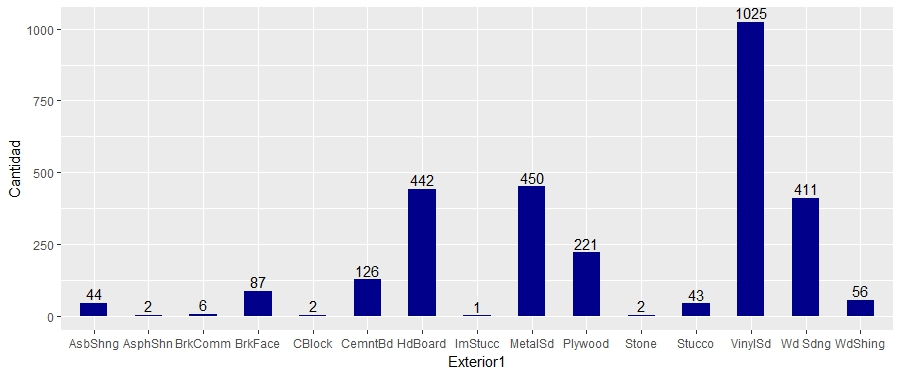
\includegraphics[scale=0.75]{Exterior1.JPEG}
	\label{p1}
	\caption{Exterior1}
\end{figure}

\begin{figure}[h]
	\centering
	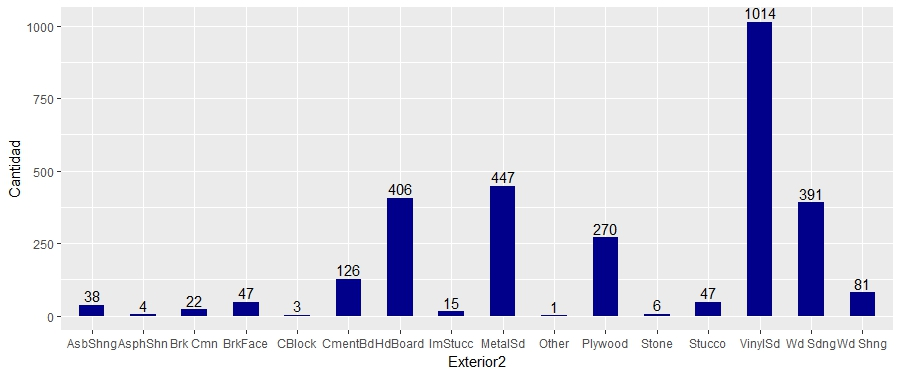
\includegraphics[scale=0.75]{Exterior2.JPEG}
	\label{p1}
	\caption{Exterior2}
\end{figure}

Ahora rellenemos los valores faltantes.\\

\begin{lstlisting}[frame=single]
f[2152,c('Exterior1st','Exterior2nd')]<-'VinylSd'
\end{lstlisting}
\vspace{2mm}

\item[2.14] \textbf{\underline{Electrical}}\\

El sistema eléctrico tiene un solo valor faltante, veamos en que fila se encuentra y rellenemosla con el valor mas frecuente.\\

\begin{lstlisting}[frame=single]
which(is.na(f$Electrical))
\end{lstlisting}

\begin{lstlisting}[frame=single]
[1] 1380
\end{lstlisting}

\begin{figure}[h]
	\centering
	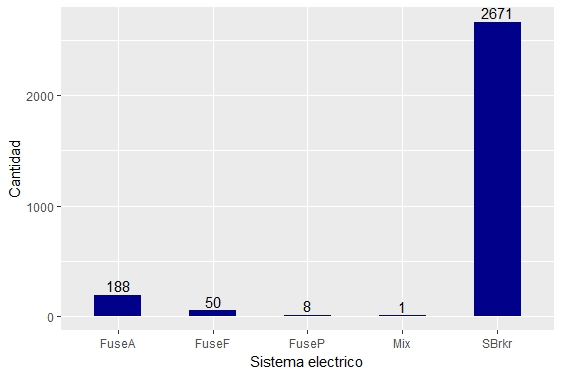
\includegraphics[scale=0.8]{Electrico.JPEG}
	\label{p1}
	\caption{Electrical}
\end{figure}

\begin{lstlisting}[frame=single]
f[1380,'Electrical']<-'SBrkr'
\end{lstlisting}
\vspace{2mm}

\item[2.15] \textbf{\underline{KitchenQual}}\\

Haremos lo mismo que en la variable Electrical.\\

\begin{lstlisting}[frame=single]
which(is.na(f$KitchenQual))
\end{lstlisting}

\begin{lstlisting}[frame=single]
[1] 1556
\end{lstlisting}

\begin{figure}[h]
	\centering
	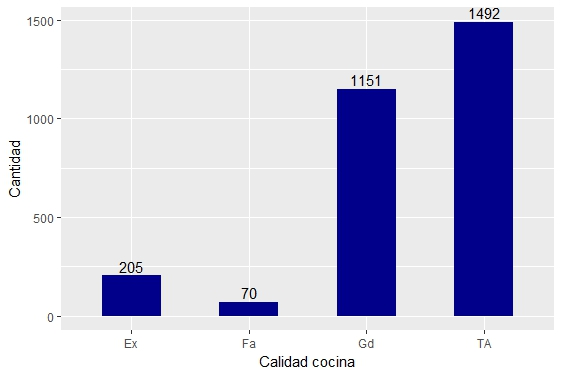
\includegraphics[scale=0.8]{Ccocina.JPEG}
	\label{p1}
	\caption{KitchenQual}
\end{figure}

\begin{lstlisting}[frame=single]
f[1556,'KitchenQual']<-'TA'
\end{lstlisting}
\vspace{2mm}

\newpage
\item[2.16] \textbf{\underline{SaleType}}\\

La variable SaleType tiene un solo valor faltante, para esto vamos a compararlo con la condición de venta para poder rellenar este valor. Veamos donde esta ubicado el valor faltante y la frecuencia de los valores de SaleType.\\

\begin{lstlisting}[frame=single]
which(is.na(f$SaleType))
\end{lstlisting}

\begin{lstlisting}[frame=single]
[1] 2490
\end{lstlisting}
\vspace{2mm}

Veamos los valores mas frecuente de la variable SaleType.\\

\begin{figure}[h]
	\centering
	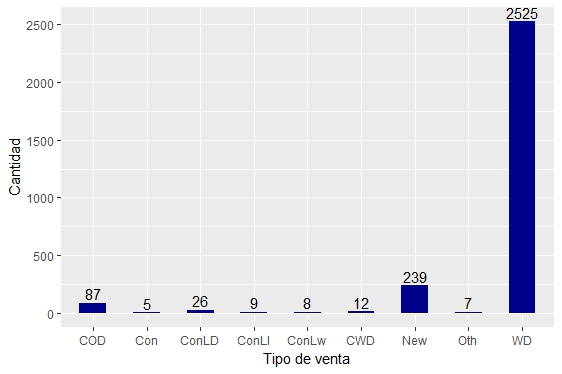
\includegraphics[scale=0.8]{Tventa.JPEG}
	\label{p1}
	\caption{SaleType}
\end{figure}

Comparemos SaleType con SaleCondition.\\

\begin{lstlisting}[frame=single]
[1] f[which(is.na(f$SaleType)),'SaleCondition']

[2] table(f$SaleCondition,f$SaleType)
\end{lstlisting}

\begin{lstlisting}[frame=single]
[1] Normal

[2]          COD  Con ConLD ConLI ConLw  CWD  New  Oth   WD
Abnorml       46    0     3     2     0    1    0    5  133
AdjLand        0    0     0     0     0    0    0    0   12
Alloca         0    0     0     0     0    0    0    0   24
Family         2    0     1     2     1    1    0    1   38
Normal        39    4    21     5     7   10    0    1 2314
Partial        0    1     1     0     0    0  239    0    4
\end{lstlisting}

\begin{lstlisting}[frame=single]
f[2490,'SaleType']<-'WD'
\end{lstlisting}

\end{itemize}
\end{itemize}

\newpage


\item \textbf{\large{\underline{Análisis Exploratorio}}}
\vspace{2mm}

Ahora que rellenamos los valores faltantes vamos a añadir columnas que son la representación númerica de algunas variables categóricas, ya que queremos que la mayoría de las variables sean númericas para tomar la mayor información posible para que nuestro modelo sea lo más preciso y ver cuales son las que tienen mayor relación con SalePrice.\\

Comenzaremos con las variables 'ExterQual','ExterCond','GarageQual','GarageCond','FireplaceQu','KitchenQual' 'HeatingQC','BsmtQual','BsmtCond','PoolQC' cuyas caracteristicas son iguales 'Ex','Gd','Ta','Fa','Po' y NA y le implementamos una escala de 0 hasta 5 a todas estas en unas nuevas variables.\\

Analogamente lo hicimos con las variables BsmtExposure, BsmtFintype1, BsmtFinType2, Functional y GarageFinish.\\

Ahora nos preguntamos si el vecindario influye en el precio de las viviendas, veamos el promedio de precios por cada vecindario.\\

\begin{lstlisting}[frame=single]
N<-f[order(f$Neighborhood),c('Neighborhood','SalePrice')]
N1<-N[!is.na(N$SalePrice),]
N2<-aggregate(N1[,2],list(N1$Neighborhood),mean)
colnames(N2)<-c('Neighborhood','Media')
N2
\end{lstlisting}

\begin{lstlisting}[frame=single]
          Neighborhood     Media
   1       Blmngtn       194870.88
   2       Blueste       137500.00
   3        BrDale       104493.75
   4       BrkSide       124834.05
   5       ClearCr       212565.43
   6       CollgCr       197965.77
   7       Crawfor       210624.73
   8       Edwards       128219.70
   9       Gilbert       192854.51
   10       IDOTRR       100123.78
   11      MeadowV        98576.47
   12      Mitchel       156270.12
   13        NAmes       145847.08
   14      NoRidge       335295.32
   15      NPkVill       142694.44
   16      NridgHt       316270.62
   17       NWAmes       189050.07
   18      OldTown       128225.30
   19       Sawyer       136793.14
   20      SawyerW       186555.80
   21      Somerst       225379.84
   22      StoneBr       310499.00
   23        SWISU       142591.36
   24       Timber       242247.45
   25      Veenker       238772.73
\end{lstlisting}

\newpage

\begin{figure}[h]
	\centering
	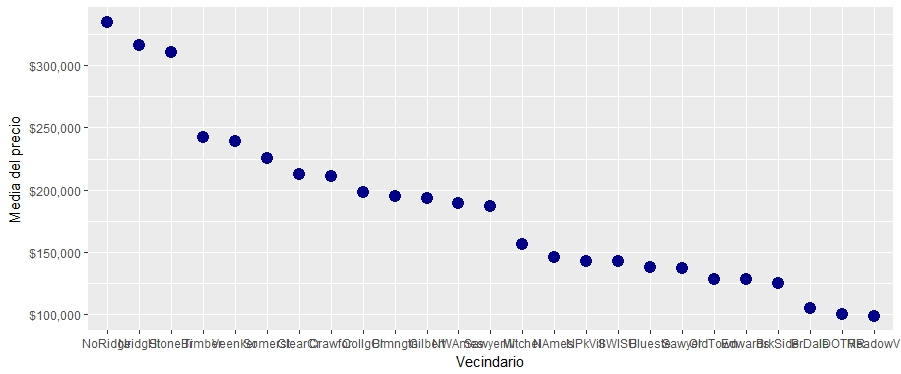
\includegraphics[scale=0.75]{Vecindario.JPEG}
	\label{p1}
	\caption{Neighborhood}
\end{figure}

Luego lo que haremos es sacar los datos númericos y veamos la correlación de estas variables númericas con SalePrice.\\

\begin{lstlisting}[frame=single]
f_numeric<-f[names(which(sapply(f, is.numeric)))]
\end{lstlisting}

\begin{lstlisting}[frame=single]
correlaciones<-cor(f_numeric[1:1460,])

cor.SalePrice<-as.matrix(sort(correlaciones[,'SalePrice'], decreasing = TRUE))
t<-names(which(apply(cor.SalePrice,1,function(x)(x>0.5))))

corrplot(correlaciones[t,t],type = 'upper',method = 'color',
cl.cex = 0.7,tl.cex=0.7,addCoef.col = 'black')
\end{lstlisting}
  
 \newpage
  
\begin{figure}[h]
	\centering
	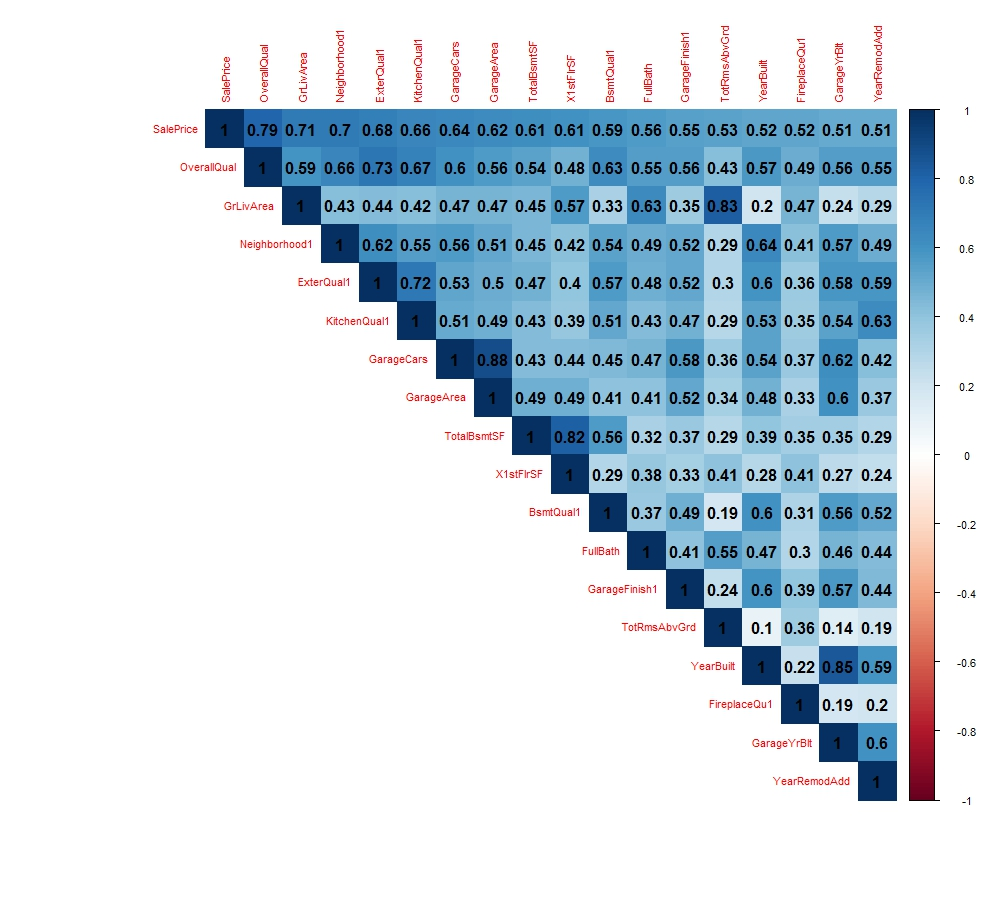
\includegraphics[scale=0.65]{Correlaciones.JPEG}
	\label{p1}
	\caption{Correlaciones}
\end{figure}

\begin{itemize}
\item[*] \textbf{\underline{Modelo}}\\

El modelo que aplicaremos a este problema es lm, lo primero que haremos es dividir nuestra data de entrenamiento en 70\% para entrenar nuestro modelo y luego predecir el 30\% restante.Esto es para ver la precisión de nuestro modelo y también porque en principio no tenemos los valores originales de los precios de las viviendas con respecto a todas las variables en la data de prueba, veamos como se comporta nuestro modelo.\\

\begin{lstlisting}[frame=single]
f_numeric<-f[names(which(sapply(f, is.numeric)))]

fn1<-f_numeric[1:1460,]
E1<-sample(1:1460,1022)
entrenamiento1<-fn1[E1,]
prueba1<-fn1[-E1,]

modelo1<-lm(SalePrice~.,entrenamiento1)
\end{lstlisting}

\begin{lstlisting}[frame=single]
p1<-predict(modelo1,prueba1)

error<-prueba1$SalePrice-p1
rmse<-function(error){sqrt(mean(error^2))}

count=0
for (i in 1:438) {
if (abs(error[i])<=10000){count = count +1}
else{count = count}

}

rmse(error)
count
\end{lstlisting}

\begin{lstlisting}[frame=single]
[1] 29453.18

[2] 152
\end{lstlisting}
\vspace{2mm}

Esto significa que tenemos un error cuádratico medio de 29.453\$ que representa un error de mas del 16\% con respecto al promedio de los precios de la vivienda y para un error menor a 10.000\$ tenemos que de 438 viviendas, 152 caen en ese rango, lo que representa una efectividad del 34\% para nuestro modelo.\\

Ahora probemos nuestro modelo para predecir la data de prueba que en principio es nuestro objetivo principal, tomamos una data de referencia dada por \url{www.kaggle.com} que predicen el precio de las viviendas para solo cuatro variables que son el año y mes de venta,número de habitaciones y el área de esta.\\

\begin{lstlisting}[frame=single]
modelo<-lm(SalePrice~.,f_numeric[1:1460,])
p3<-predict(modelo,newdata=f_numeric[1461:2919,])
p4<-as.matrix(p3)

error1<-referencia$SalePrice-p3

rmse(error1)

count1=0
for (i in 1:1459) {
if (abs(error1[i])<=10000){count1 = count1 +1}
else{count1 = count1}

}

rmse(error1)
count1
\end{lstlisting}

\begin{lstlisting}[frame=single]
[1] 71437.27

[2] 136
\end{lstlisting}
\vspace{2mm}

Esto significa que 136 viviendas caen dentro del rango de un error menor a 10.000\$ lo cual representa el 9\% de precision con respecto a la data de referencia.\\
\end{itemize}

\newpage

\item \textbf{\underline{Análisis Final}}
\vspace{2mm}

Como vimos anteiormente nuestra pregunta mas importante de predecir los precios de las viviendas fueron respondidas, ahora veremos las distribuciones de los precios que hemos predicho para observar si estas tienen un comportamiento similar a los precios de la data de entrenamiento.\\


\begin{figure}[h]
	\centering
	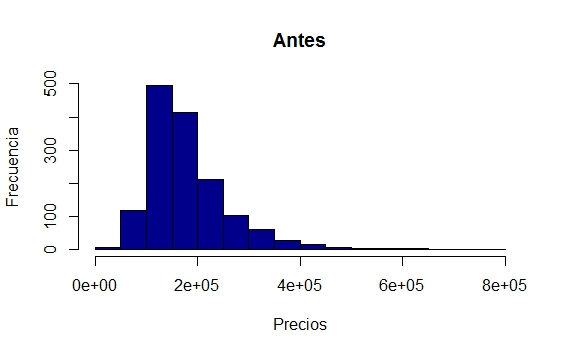
\includegraphics[scale=0.8]{Precios1.JPEG}
	\label{p1}
	\caption{SalePrice}
\end{figure}

\begin{figure}[h]
	\centering
	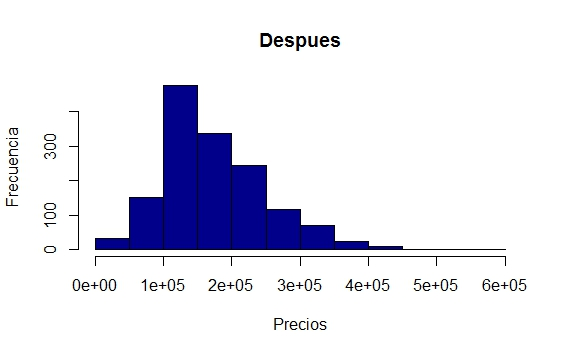
\includegraphics[scale=0.8]{Precios2.JPEG}
	\label{p1}
	\caption{SalePrice}
\end{figure}

¿Qué aprendimos de los datos?,Tomarse el tiempo necesario para indagar los datos te generan un conocimiento y te ayuda a interpretar mejor los resultados del problemas que se este trabajando, ya que sin el debido análisis y limpieza que estos requieren nos crean márgenes de errores muy grandes y pérdida de tiempo.











\end{itemize}
\end{document}